\documentclass{rapportENSIAS}
\usepackage{lipsum}
\usepackage{minted}
\definecolor{bg}{rgb}{0.95,0.95,0.95} % Adjust the RGB values as needed
\usepackage{graphicx}  % Pour les images
\usepackage{booktabs}  % Pour les jolis tableaux
\usepackage{xcolor}    % Pour les couleurs (Rouge/Vert)
\usepackage{float}     % Pour forcer le placement des images (H)

\usepackage{titlesec} % For customizing chapter and section titles
\usepackage{tocloft} % For customizing the table of contents
\usepackage{hyperref} % For adding hyperlinks
\usepackage{tikz}               % Pour dessiner le Sitemap
\usetikzlibrary{shapes,arrows,positioning,shadows}
\usepackage{colortbl}           % Pour colorer les cellules du tablea 
\definecolor{ensiasBlue}{RGB}{44, 62, 80} % Bleu ENSIAS (Optionnel)
\definecolor{lightGray}{RGB}{240, 240, 240}
% Désactiver les messages problématiques de tocbasic
\PassOptionsToPackage{messages=off}{tocbasic}

% OU mettre cette ligne avant \usepackage{nomencl}
\RequirePackage{scrlfile}
\PreventPackageFromLoading{tocbasic}

\usepackage{nomencl}


\title{Rapport ENSIAS - Template} %Titre du fichier

\begin{document}

%----------- Informations du rapport ---------

\titre{Titre du rapport} %Titre du fichier .pdf
%\UE{UE PRO} %Nom de la UE
\sujet{Projet de Fin d'Année} %Nom du sujet

\enseignant{Prénom \textsc{Nom}} %Nom de l'enseignant

\eleves{Saad \textsc{ALAOUI SOSSE} \\
		Med Chadi \textsc{TAQI} \\ 
        Chaymae \textsc{BOUAZZA} \\ 
		Imane \textsc{BENABBOU} } 

\jury{ DR B. \textsc{BERRADA}\\ 
    }

%----------- Initialisation -------------------
        
\fairemarges %Afficher les marges
\fairepagedegarde % Créer la page de garde

%--------------les premiers pages--------------
\chapter*{Remerciements}
\chapter*{Remerciements}
\addcontentsline{toc}{chapter}{Dédicaces et Remerciements}

\vspace{1.5cm}

Au seuil de ce travail, il nous est agréable d'exprimer notre reconnaissance à tous ceux qui ont contribué à son élaboration.

Nous tenons tout d'abord à exprimer notre profonde gratitude et notre grand respect à notre professeur et encadrant, \textbf{Dr. BERRADA}. La qualité de son enseignement dans le module d'\textbf{Interaction Homme-Machine (IHM)} a été la pierre angulaire de ce projet. Ses directives précieuses et son expertise en ergonomie logicielle ont guidé notre réflexion pour placer l'utilisateur au centre de notre conception.

Nous le remercions également, ainsi que saprécense comme membre du jury, pour l'honneur qu'ils nous fait d'évaluer notre travail. Nous sommes conscients de l'exigence académique qu'elle représente et nous espérons être à la hauteur de sa confiance.

Nous saisissons cette occasion pour remercier tout le corps professoral de l'\textbf{ENSIAS} pour la qualité de la formation dispensée, ainsi que l'ensemble du personnel administratif pour leur dévouement constant.

Enfin, aucune œuvre ne peut s'accomplir sans le soutien inconditionnel de nos proches. Nous dédions ce modeste travail à nos parents, pour leurs sacrifices et leurs prières, ainsi qu'à nos amis et collègues de promotion, pour l'esprit de fraternité et d'entraide qui a marqué ce semestre.

\vspace{2cm} % modifier dans le fichier 
\newpage
\section*{Résumé}

Dans un contexte urbain où la mobilité est souvent synonyme de friction et de stress cognitif, ce projet explore la refonte numérique de l'expérience de transport public. L'objectif principal n'était pas seulement de digitaliser un service, mais de concevoir une \textbf{Interaction Homme-Machine (IHM)} capable de rassurer l'usager et de simplifier ses décisions.

En adoptant une démarche de \textbf{Conception Centrée Utilisateur (CCU)}, nous avons d'abord modélisé les modèles mentaux de nos usagers à travers des Personas (de l'étudiante experte au touriste désorienté). Cette phase d'analyse a guidé le design de nos interfaces, privilégiant l'affordance, le feedback immédiat et la minimisation de la charge mentale.

Le résultat est un prototype haute fidélité articulé autour de deux axes ergonomiques : la visualisation spatiale en temps réel (pour combler le besoin de réassurance) et la linéarisation du parcours d'achat (pour éliminer les obstacles transactionnels). Ce rapport démontre comment une interface bien pensée peut transformer une contrainte quotidienne en une expérience fluide.

\vspace{0.5cm}
\textbf{Mots-clés :} IHM, Expérience Utilisateur (UX), Design Thinking, Personas, Prototypage, Affordance, Mobilité Intelligente.

\vspace{1cm}

\newpage
\chapter*{Introduction générale}
\addcontentsline{toc}{chapter}{Introduction générale}
% intro
%------------
\newpage
\tabledematieres %Créer la table de matières

\newpage
\listoffigures

\newpage
\listoftables


%------------ Corps du rapport ----------------
\chapter{Phase d'Empathie \& Recherche (Comprendre)}

% ==============================================================================
% 1. CONTEXTE & PRESENTATION
% ==============================================================================
\section{Contexte : L'Optimisation par l'IHM}

Le projet \textbf{UrbanMove} s'inscrit dans une démarche d'\textbf{optimisation d'un existant}. Le réseau de transport actuel dispose déjà d'une infrastructure technique fonctionnelle (flotte de bus, capteurs GPS, API backend), mais souffre d'un déficit majeur d'adoption dû à une interface utilisateur obsolète, voire inexistante.

Notre mission n'est pas de refondre le code métier (backend), mais de concevoir une \textbf{couche d'interaction (Frontend/IHM)} capable de valoriser ces données pour l'usager. L'objectif est de passer d'un système "fonctionnel" à un système "utilisable et désirable".

\section{Présentation du Projet UrbanMove : Une couche d'interaction unifiée}

Le projet \textbf{UrbanMove} ne se définit pas comme une simple application de billettique, mais comme une plateforme de **Mobilité en tant que Service (MaaS)**. Dans un contexte où l'infrastructure technique (flotte de bus, capteurs GPS, API de calcul d'itinéraire) préexistait mais restait inexploitée faute d'interface, UrbanMove vient se greffer comme la \textbf{couche d'interaction} (Frontend) indispensable pour valoriser ces données.

L'ambition est de transformer une infrastructure "passive" en un service "proactif" et centré sur l'utilisateur, à travers deux interfaces distinctes mais interconnectées.

\subsection{L'Écosystème UrbanMove}

Le système repose sur une architecture duale, répondant à deux besoins contradictoires : la simplicité pour le grand public et la densité d'information pour les gestionnaires.

\subsubsection{1. Le Module Passager (Application Mobile)}
Il s'agit du point de contact unique pour l'usager. Conçue pour une utilisation en mobilité ("On-the-go"), cette interface vise à réduire la charge cognitive liée au voyage. Elle intègre trois piliers fonctionnels :
\begin{itemize}
    \item \textbf{Information Voyageur Temps Réel (IVTR) :} Contrairement aux fiches horaires statiques, l'application interroge les capteurs GPS existants pour afficher la position exacte des bus sur une carte interactive, supprimant l'incertitude de l'attente.
    \item \textbf{Dématérialisation (M-Ticketing) :} Le module d'achat permet l'acquisition instantanée de titres (unitaires ou abonnements) et génère un \textbf{QR Code dynamique} pour la validation, supprimant la gestion des espèces à bord.
    \item \textbf{Guidage Assisté :} Un planificateur d'itinéraire multimodal qui suggère les correspondances optimales en fonction du trafic.
\end{itemize}

\subsubsection{2. Le Module Administration (Dashboard Web)}
Destiné aux régulateurs et gestionnaires du réseau, ce tableau de bord transforme les données brutes du backend en outils d'aide à la décision. Il permet :
\begin{itemize}
    \item \textbf{La Supervision (Monitoring) :} Visualisation globale de la flotte, état de santé des bus et alertes en cas de retard critique.
    \item \textbf{La Gestion Commerciale :} Création de nouvelles lignes, modification des tarifs et gestion des comptes utilisateurs.
    \item \textbf{L'Analyse de Données (Business Intelligence) :} Des graphiques détaillés sur les revenus par ligne et les pics d'affluence, permettant d'adapter l'offre à la demande.
\end{itemize}

\subsection{Objectifs de l'Optimisation IHM}

Le défi technique de ce projet ne résidait pas dans la logique métier (déjà gérée par des microservices Spring Boot), mais dans l'\textbf{utilisabilité}. L'intervention IHM a visé trois objectifs de performance :

\begin{enumerate}
    \item \textbf{Réduction de la Frictionalité :} Passer de 5 étapes pour acheter un ticket (guichet physique) à 3 "taps" sur l'écran (Loi de Fitts).
    \item \textbf{Feedback Système Immédiat :} Fournir une confirmation visuelle ou haptique pour chaque action critique (paiement validé, bus en approche), appliquant ainsi la première heuristique de Nielsen (Visibilité de l'état du système).
    \item \textbf{Accessibilité Universelle :} Concevoir des interfaces contrastées et lisibles, adaptées aussi bien aux étudiants pressés qu'aux usagers occasionnels peu technophiles.
\end{enumerate}

\subsection{Positionnement de la solution}
En résumé, UrbanMove agit comme le \textbf{liant numérique} entre une infrastructure physique complexe et un usager en quête de simplicité. Là où l'ancien système se contentait de "faire rouler des bus", la nouvelle interface UrbanMove promet de "piloter une expérience de voyage".

% ==============================================================================
% 3. METHODOLOGIE & ANALYSE DETAILLEE
% ==============================================================================
\section{Analyse Quantitative Détaillée : La Voix de l'Utilisateur}

Pour garantir la pertinence de cette refonte IHM, nous avons adopté la méthode du \textbf{Design Thinking}. Cette phase d'Empathie s'appuie sur une enquête quantitative rigoureuse menée auprès de \textbf{29 participants}. Nous analysons ici chaque question pour en extraire une directive de conception IHM.

% --- Q1 AGE ---
\subsection{Q1. Tranche d'âge : Une cible "Digital Native"}
\textbf{Données :} 58,6 \% des répondants ont entre 18 et 25 ans, et 20,7 \% ont moins de 18 ans.
\newline
\textbf{Analyse :} La quasi-totalité de nos utilisateurs (près de 80\%) est née avec le numérique. Ils sont habitués aux standards UX élevés des géants du web (Uber, Instagram).
\newline
\textbf{Implication IHM :} L'interface doit être fluide, réactive et privilégier le "Mobile First". Le mode sombre (Dark Mode) est une fonctionnalité attendue par cette cible.

\begin{figure}[H]
    \centering
    \includegraphics[width=0.8\textwidth]{imgs/graph_age.png}
    \caption{Q1 : Répartition démographique jeune}
\end{figure}

% --- Q2 DIFFICULTES CONDUCTEUR ---
\subsection{Q2. Difficultés Métier : Le besoin de visibilité}
\textbf{Données :} 57,1 \% des gestionnaires citent le "Manque de visibilité en temps réel sur la position des bus" comme difficulté majeure. La gestion de la monnaie est aussi un irritant.
\newline
\textbf{Analyse :} Les opérateurs sont aveugles. Ils gèrent le réseau "à l'instinct" sans données fiables.
\newline
\textbf{Implication IHM (Admin) :} Le Dashboard ne doit pas être un tableur Excel. Il doit offrir une \textbf{Carte de Supervision} en temps réel pour piloter la flotte visuellement.

\begin{figure}[H]
    \centering
    \includegraphics[width=0.8\textwidth]{imgs/graph_cond_frust.png}
    \caption{Q2 : Les angles morts de la gestion actuelle}
\end{figure}

% --- Q3 ROLE ---
\subsection{Q3. Rôle : L'équilibre Expert / Novice}
\textbf{Données :} Égalité parfaite (37,9 \%) entre les usagers Quotidiens (Experts) et Occasionnels (Novices).
\newline
\textbf{Analyse :} L'application doit servir deux maîtres. L'expert veut aller vite, le novice veut être rassuré.
\newline
\textbf{Implication IHM :} Conception d'une navigation "Dual-Mode". Des raccourcis "Favoris" en un clic pour les habitués, et un moteur de recherche d'itinéraire guidé pas-à-pas pour les nouveaux.

\begin{figure}[H]
    \centering
    \includegraphics[width=1\textwidth]{imgs/graph_role.png}
    \caption{Q3 : Répartition des profils d'usage}
\end{figure}

% --- Q4 FREQUENCE ---
\subsection{Q4. Fréquence : Un outil du quotidien}
\textbf{Données :} 41,4 \% utilisent le bus "Tous les jours".
\newline
\textbf{Analyse :} L'application sera ouverte plusieurs fois par jour. La moindre friction (temps de chargement, clic inutile) deviendra insupportable à la longue.
\newline
\textbf{Implication IHM :} Optimisation de la performance (Loi de Doherty : réponse < 400ms) et persistance de la session (pas de reconnexion à chaque fois).

\begin{figure}[H]
    \centering
    \includegraphics[width=1\textwidth]{imgs/graph_freq.png}
    \caption{Q4 : Intensité d'usage}
\end{figure}

% --- Q5 SATISFACTION ---
\subsection{Q5. Satisfaction Actuelle : L'urgence du changement}
\textbf{Données :} 48,1 \% sont "Très insatisfaits" (Note 1/5) de l'achat physique.
\newline
\textbf{Analyse :} Le système de billettique actuel est le point noir de l'expérience. C'est un irritant majeur.
\newline
\textbf{Implication IHM :} Le module d'achat (M-Ticket) doit être la fonctionnalité la plus accessible, placée au centre de la barre de navigation (Tab Bar).

\begin{figure}[H]
    \centering
    \includegraphics[width=0.9\textwidth]{imgs/graph_satis.png}
    \caption{Q5 : Rejet massif de la billettique physique}
\end{figure}

% --- Q6 FRUSTRATIONS ---
\subsection{Q6. Frustrations : Le stress de l'inconnu}
\textbf{Données :} "Incertitude horaire" et "Manque de visibilité géographique" sont cités par 58,6 \% des usagers.
\newline
\textbf{Analyse :} L'usager ne déteste pas attendre, il déteste \textit{ne pas savoir combien de temps} il va attendre.
\newline
\textbf{Implication IHM :} Affichage proéminent du "Temps d'attente réel" (et non théorique) avec un code couleur (Vert = À l'heure, Rouge = Retard).

\begin{figure}[H]
    \centering
    \includegraphics[width=0.9\textwidth]{imgs/graph_frust.png}
    \caption{Q6 : Les facteurs de stress}
\end{figure}

% --- Q7 & Q8 IMPORTANCE ---
\subsection{Q7 \& Q8. Attentes : Plébiscite pour le Digital}
\textbf{Données :} L'achat In-App et la Géolocalisation obtiennent des scores d'importance supérieurs à 4.2/5.
\newline
\textbf{Analyse :} Il y a une forte demande (Market Pull) pour ces fonctionnalités. Ce ne sont pas des gadgets, mais des prérequis.
\newline
\textbf{Implication IHM :} Ces deux fonctionnalités doivent constituer le cœur de l'expérience (Core Features).

\begin{figure}[H]
    \centering
    \includegraphics[width=0.8\textwidth]{imgs/graph_sol.png}
    \includegraphics[width=0.8\textwidth]{imgs/graph_rating.png}
    \caption{Q7/Q8 : Validation de la proposition de valeur}
\end{figure}

% --- Q9 SCENARIOS ---
\subsection{Q9. Scénarios Futurs : La demande de proactivité}
\textbf{Données :} Le scénario "Notification 5 min avant l'arrivée" reçoit les meilleures notes.
\newline
\textbf{Analyse :} L'utilisateur veut une application qui "veille" pour lui, plutôt que de devoir vérifier sa montre toutes les 30 secondes.
\newline
\textbf{Implication IHM :} Intégration d'un système de \textbf{Push Notifications} intelligent et contextuel.

\begin{figure}[H]
    \centering
    \includegraphics[width=1\textwidth]{imgs/graph_solus.png}
    \caption{Q9 : Préférence pour l'assistance proactive}
\end{figure}

% --- Q10 OUTILS ---
\subsection{Q10. Outils Métier : Efficacité opérationnelle}
\textbf{Données :} 66,7 \% demandent la "Validation simplifiée".
\newline
\textbf{Analyse :} Le conducteur ne doit pas perdre de temps à contrôler des écrans complexes.
\newline
\textbf{Implication IHM :} Interface conducteur épurée avec un gros bouton "SCAN" et un feedback sonore (Bip valide / Bip invalide).

\begin{figure}[H]
    \centering
    \includegraphics[width=0.9\textwidth]{imgs/graph_condu.png}
    \caption{Q10 : Priorités pour l'interface conducteur}
\end{figure}

% ==============================================================================
% 4. SYNTHESE
% ==============================================================================
\section{Synthèse : Matrice de Transition (Data $\rightarrow$ Design)}

Cette analyse exhaustive nous permet de dresser la liste définitive des besoins fonctionnels et de leurs traductions en composants d'interface.

\begin{table}[H]
    \centering
    \renewcommand{\arraystretch}{1.5}
    \begin{tabular}{@{}p{4cm} p{4cm} p{8.5cm}@{}}
        \toprule
        \textbf{Source (Question)} \& \textbf{Besoin Identifié}   \& \textbf{Traduction IHM (Composant)} \\
        \midrule
        Q6 (Incertitude) \& Réassurance temporelle \& \textbf{Carte Live} avec icônes de bus en mouvement et décompte temps réel. \\
        \midrule
        Q5 (Achat) \& Autonomie \& \textbf{Store In-App} avec tunnel de paiement simplifié (3 étapes max). \\
        \midrule
        Q3 (Habitude) \& Rapidité d'accès \& \textbf{Widget "Favoris"} sur l'écran d'accueil pour lancer un trajet en 1 tap. \\
        \midrule
        Q9 (Notification) \& Assistance proactive \& \textbf{Alertes Push} "Votre bus arrive dans 5 min". \\
        \midrule
        Q2/Q10 (Métier) \& Supervision \& \textbf{Dashboard Admin} avec vue "Tour de contrôle" et Scan QR rapide. \\
        \bottomrule
    \end{tabular}
    \caption{Matrice de transition : Du problème à la solution IHM}
    \label{tab:transition}
\end{table}

\section*{Conclusion du Chapitre}

L'enquête a permis de dépasser les simples suppositions. Nous savons désormais précisément \textit{pour qui} nous concevons (des jeunes connectés et pressés) et \textit{quoi} concevoir (une app de temps réel et de billettique). Ces données fondatrices nous permettent de modéliser nos \textbf{Personas} au chapitre suivant, qui incarneront ces statistiques dans des profils humains tangibles.
\chapter{Phase de Définition (Analyser)}

\section{Nos Personas (Les Archétypes Validés)}

Pour incarner les besoins identifiés lors de la recherche, nous avons défini quatre profils utilisateurs : le cœur de cible (l'étudiante), le cas de rupture (l'automobiliste), l'opérationnel (le conducteur) et l'utilisateur externe (le touriste).

% --- PERSONA 1 : L'ÉTUDIANTE ---
\subsection{Persona 1 : Safae, "L'Étudiante Pressée"}
\textit{Le profil régulier (Daily Commuter) - 21 ans.}

\begin{figure}[H]
    \centering
    % Insérez ici l'image de la fiche ou la photo
    \includegraphics[width=1.1\linewidth]{imgs/safae.png}
\end{figure}

\begin{itemize}
    \item \textbf{Bio \& Contexte :} Safae prend le bus tous les jours à 7h30 pour aller à l'ENSIAS. "Digital Native", elle gère tout depuis son smartphone. Elle ne tolère pas l'attente injustifiée et oublie souvent son portefeuille (mais jamais son téléphone).
    \item \textbf{Buts (Goals) :}
    \begin{itemize}
        \item Connaître l'heure d'arrivée exacte du bus (Real-time).
        \item Gérer son abonnement mensuel directement sur l'appli.
        \item Utiliser son téléphone comme titre de transport.
    \end{itemize}
    \item \textbf{Frustrations (Pains) :}
    \begin{itemize}
        \item Le stress du "Bus fantôme" (pas d'info).
        \item Les files d'attente pour recharger sa carte physique.
        \item La peur d'être en retard en cours.
    \end{itemize}
\end{itemize}
\clearpage
% --- PERSONA 2 : L'AUTOMOBILISTE ---
\subsection{Persona 2 : Sarah, "L'Automobiliste Anxieuse"}
\textit{Le cas de rupture (Utilisateur occasionnel) - 31 ans.}

\begin{figure}[H]
    \centering
    \includegraphics[width=1.1\linewidth]{imgs/automobiliste.png}
\end{figure}

\begin{itemize}
    \item \textbf{Bio \& Contexte :} Sarah ne prend jamais le bus. Suite à une panne de voiture, elle doit l'utiliser en urgence. Elle n'a pas d'espèces ("Cashless") et ne connaît pas les lignes. Elle est en situation de stress et d'anxiété sociale.
    \item \textbf{Buts (Goals) :}
    \begin{itemize}
        \item Être guidée pas-à-pas comme avec un GPS.
        \item Payer sans contact (Apple Pay/Carte) pour éviter la gestion de la monnaie.
        \item Se rassurer en voyant le bus avancer sur la carte.
    \end{itemize}
    \item \textbf{Frustrations (Pains) :}
    \begin{itemize}
        \item Ne pas avoir de monnaie pour payer le chauffeur.
        \item La peur de se tromper de direction ou de rater l'arrêt.
        \item Le sentiment d'être une "touriste" dans sa propre ville.
    \end{itemize}
\end{itemize}
\clearpage
% --- PERSONA 3 : LE CONDUCTEUR ---
\subsection{Persona 3 : Ayoub, "Le Conducteur / Staff"}
\textit{L'Admin terrain et garant de l'efficacité - 31 ans.}

\begin{figure}[H]
    \centering
    \includegraphics[width=1.1\linewidth]{imgs/chauffeur.png}
\end{figure}

\begin{itemize}
    \item \textbf{Bio \& Contexte :} Chauffeur expérimenté, Ayoub aime conduire mais est usé par la gestion de la caisse à bord qui crée des retards. Il veut se concentrer sur la route, pas sur la comptabilité.
    \item \textbf{Buts (Goals) :}
    \begin{itemize}
        \item Fluidifier la montée des passagers (Validation autonome).
        \item Recevoir son itinéraire et les alertes sur sa tablette.
        \item Signaler un incident en un clic (Gros bouton).
    \end{itemize}
    \item \textbf{Frustrations (Pains) :}
    \begin{itemize}
        \item Les disputes liées au rendu de monnaie.
        \item Les appels téléphoniques de la régulation pendant la conduite.
        \item Ne pas savoir s'il est en retard sur son horaire.
    \end{itemize}
\end{itemize}
\clearpage
% --- PERSONA 4 : LE TOURISTE ---
\subsection{Persona 4 : Manuel, "Le Touriste Explorateur"}
\textit{Le besoin de simplicité et de paiement international - 39 ans.}

\begin{figure}[H]
    \centering
    \includegraphics[width=1.1\linewidth]{imgs/touriste_fiche.png}
\end{figure}

\begin{itemize}
    \item \textbf{Bio \& Contexte :} Visiteur étranger présent pour 3 jours. Il ne parle pas la langue et ne veut pas retirer de cash. Il veut visiter les monuments ("Tour Hassan") sans se soucier de la complexité du réseau.
    \item \textbf{Buts (Goals) :}
    \begin{itemize}
        \item Payer avec sa carte internationale in-app.
        \item Sélectionner des points d'intérêt touristiques sur la carte.
        \item Être géolocalisé pour ne pas se perdre.
    \end{itemize}
    \item \textbf{Frustrations (Pains) :}
    \begin{itemize}
        \item La barrière de la langue avec le chauffeur.
        \item La complexité des zones tarifaires.
        \item L'obligation d'avoir de la monnaie locale.
    \end{itemize}
\end{itemize}

\section{Carte d'Empathie (Empathy Map)}

Focus sur notre cœur de cible, \textbf{Safae (L'Étudiante)}, lors de l'attente à l'arrêt.

\begin{table}[H]
    \centering
    \begin{tabular}{|p{0.45\textwidth}|p{0.45\textwidth}|}
        \hline
        \textbf{Ce qu'elle VOIT (See)} \& \textbf{Ce qu'elle ENTEND (Hear)} \\
        \begin{itemize}
            \item Le bus partir au loin.
            \item Une foule qui attend.
            \item Des panneaux horaires vides.
        \end{itemize} \& 
        \begin{itemize}
            \item Les gens souffler d'impatience.
            \item Le bruit de la circulation.
            \item "Préparez la monnaie !"
        \end{itemize} \\
        \hline
        \textbf{Ce qu'elle RESSENT (Feel)} \& \textbf{Ce qu'elle FAIT (Do)} \\
        \begin{itemize}
            \item Frustration (retard).
            \item Stress (oubli de carte).
            \item Envie de transparence.
        \end{itemize} \& 
        \begin{itemize}
            \item Regarde son téléphone (compulsif).
            \item Cherche sa carte dans son sac.
            \item Se plaint sur WhatsApp.
        \end{itemize} \\
        \hline
    \end{tabular}
    \caption{Carte d'Empathie : Safae à l'arrêt}
\end{table}

\section{Définition du Problème (Problem Statement)}

L'analyse croisée de nos quatre personas met en lumière une fracture numérique critique. Le problème ne se limite pas au paiement ponctuel, mais concerne l'ensemble de l'expérience de mobilité.

Nous devons répondre simultanément aux besoins de l'usager régulier (Abonnements, Temps réel) et de l'usager occasionnel (Ticket unique, Guidage).

Nous formulons donc notre défi majeur ("How Might We") ainsi :

\begin{center}
    \fbox{\begin{minipage}{0.95\textwidth}
        \centering
        \vspace{0.4cm}
        \Large
        \textbf{\textit{"Comment pourrions-nous centraliser l'expérience de transport pour offrir une visibilité totale (Temps Réel) et une dématérialisation complète (Abonnements/Tickets) afin de supprimer le stress et le cash ?"}}
        \vspace{0.4cm}
    \end{minipage}}
\end{center}

Cette problématique se décompose en trois axes de conception pour la suite du projet :

\begin{enumerate}
    \item \textbf{L'Axe Informationnel (Réassurance) :} Comment garantir la géolocalisation précise et l'horaire en temps réel pour qu'un étudiant ou un touriste n'attende plus jamais "à l'aveugle" ?
    \item \textbf{L'Axe Transactionnel (Fluidité) :} Comment permettre l'achat instantané de tout titre de transport (du ticket unitaire à l'abonnement annuel) sans aucune interaction physique ni espèce ?
    \item \textbf{L'Axe Opérationnel (Efficacité) :} Comment réduire la charge mentale du conducteur en automatisant la validation et le guidage ?
\end{enumerate}
\chapter{Phase d'Idéation \& Conception (Concevoir)}

\section{Introduction : De la Problématique à la Solution}

Suite à la définition de notre problématique au chapitre précédent — \textit{"Comment centraliser l'expérience de transport pour supprimer le stress et le cash ?"} — nous entrons ici dans la phase de conception concrète.

Cette étape vise à traduire les besoins émotionnels de nos quatre personas (Safae, Sara, Ayoub et Manuel) en fonctionnalités techniques tangibles. Pour ce faire, nous avons adopté une approche Agile, en découpant le projet en récits utilisateurs (\textit{User Stories}) et en structurant l'information pour minimiser la friction cognitive.

\section{Définition des Fonctionnalités (User Stories)}

Afin de garantir que chaque développement apporte une valeur ajoutée réelle, nous utilisons le format BDD (\textit{Behavior Driven Development}) : \textbf{"En tant que [Persona], je veux [Action] afin de [Bénéfice]"}.

Nous avons priorisé ces fonctionnalités selon la méthode \textbf{MoSCoW} (Must have, Should have, Could have, Won't have) pour définir le périmètre de notre MVP (\textit{Minimum Viable Product}).

\begin{table}[H]
    \centering
    \renewcommand{\arraystretch}{1.6}
    \footnotesize
    \begin{tabular}{|p{0.15\textwidth}|p{0.60\textwidth}|p{0.15\textwidth}|}
        \hline
        \rowcolor{ensiasBlue!10} \textbf{Cible} \& \textbf{User Story (Format BDD)} \& \textbf{Priorité} \\
        \hline
        \textbf{Safae} \newline (L'Étudiante) \& \textbf{En tant que} passagère quotidienne, \newline \textbf{Je veux} consulter la position du bus en temps réel sur une carte, \newline \textbf{Afin d'} optimiser mon temps et ne pas attendre inutilement à l'arrêt. \& \textbf{MUST HAVE} \newline (Vital) \\
        \hline
        \textbf{Safae} \newline (L'Étudiante) \& \textbf{En tant qu'} abonnée mensuelle, \newline \textbf{Je veux} renouveler et payer mon abonnement directement dans l'application, \newline \textbf{Afin d'} éviter les files d'attente aux guichets physiques chaque début de mois. \& \textbf{MUST HAVE} \newline (Vital) \\
        \hline
        \rowcolor{ensiasBlue!10} \textbf{Sara} \newline (L'Occasionnelle) \& \textbf{En tant qu'} utilisatrice sans espèces ("Cashless"), \newline \textbf{Je veux} acheter un ticket unitaire via ma carte bancaire, \newline \textbf{Afin de} pouvoir monter à bord immédiatement sans chercher de monnaie. \& \textbf{MUST HAVE} \newline (Vital) \\
        \hline
        \textbf{Sara} \newline (L'Anxieuse) \& \textbf{En tant que} novice du réseau, \newline \textbf{Je veux} rechercher un itinéraire optimisé d'un point A à un point B, \newline \textbf{Afin de} ne pas me perdre ou me tromper de ligne. \& \textbf{SHOULD HAVE} \newline (Important) \\
        \hline
        \rowcolor{ensiasBlue!10} \textbf{Manuel} \newline (Le Touriste) \& \textbf{En tant que} visiteur étranger, \newline \textbf{Je veux} visualiser les points d'intérêt touristiques sur la carte, \newline \textbf{Afin de} choisir ma destination visuellement sans connaître les noms de quartiers. \& \textbf{COULD HAVE} \newline (Confort) \\
        \hline
        \textbf{Ayoub} \newline (Admin) \& \textbf{En tant que} gestionnaire du réseau, \newline \textbf{Je veux} créer, modifier ou supprimer des lignes et des bus (CRUD), \newline \textbf{Afin d'} adapter l'offre de transport aux changements opérationnels. \& \textbf{MUST HAVE} \newline (Back-Office) \\
        \hline
    \end{tabular}
    \caption{Matrice des User Stories priorisées pour le MVP}
    \label{tab:userstories}
\end{table}

\section{Architecture de l'Information (Sitemap)}

Avant d'entamer le design des interfaces, nous avons structuré le parcours utilisateur (\textit{User Flow}). L'objectif ergonomique est de respecter la règle des "3 clics" pour l'action la plus critique : l'achat d'un titre de transport.

Le schéma ci-dessous illustre l'arborescence de l'application mobile "Voyageur", telle qu'implémentée dans nos maquettes :

\vspace{0.5cm}

% Schéma TikZ pour le Sitemap (Navigation)
\begin{figure}[H]
    \centering
    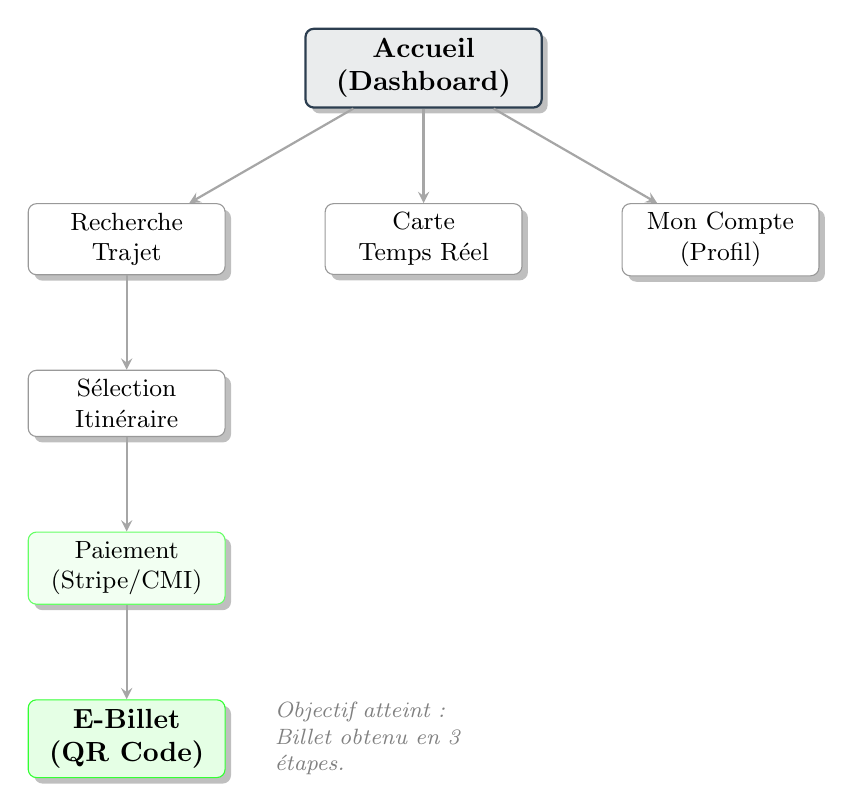
\begin{tikzpicture}[
        node distance=1.2cm and 1cm,
        box/.style={rectangle, draw=gray!80, rounded corners=3pt, fill=white, align=center, minimum height=0.8cm, minimum width=2.5cm, drop shadow, font=\small},
        root/.style={rectangle, draw=ensiasBlue, thick, rounded corners=3pt, fill=ensiasBlue!10, align=center, minimum height=1cm, minimum width=3cm, drop shadow, font=\bfseries},
        arrow/.style={->, thick, >=stealth, color=gray!70}
    ]

    % Racine
    \node[root] (home) {Accueil \\ (Dashboard)};

    % Niveau 2
    \node[box, below left=of home] (search) {Recherche \\ Trajet};
    \node[box, below=of home] (map) {Carte \\ Temps Réel};
    \node[box, below right=of home] (account) {Mon Compte \\ (Profil)};

    % Niveau 3 (Processus d'achat)
    \node[box, below=of search] (results) {Sélection \\ Itinéraire};
    \node[box, below=of results, fill=green!5, draw=green!60] (payment) {Paiement \\ (Stripe/CMI)};
    \node[box, below=of payment, fill=green!10, draw=green!80, font=\bfseries] (ticket) {E-Billet \\ (QR Code)};

    % Liens
    \draw[arrow] (home) -- (search);
    \draw[arrow] (home) -- (map);
    \draw[arrow] (home) -- (account);
    \draw[arrow] (search) -- (results);
    \draw[arrow] (results) -- (payment);
    \draw[arrow] (payment) -- (ticket);
    
    % Annotation latérale
    \node[right=0.5cm of ticket, text width=3cm, font=\footnotesize\itshape, color=gray] {Objectif atteint : \\ Billet obtenu en 3 étapes.};

    \end{tikzpicture}
    \caption{Sitemap : Parcours simplifié pour l'utilisateur}
    \label{fig:sitemap}
\end{figure}

Ce flux de navigation valide le parcours de notre persona \textbf{Sara} : elle ouvre l'application, recherche sa destination, paie, et obtient son QR Code. La complexité technique (calcul d'itinéraire, transaction bancaire) est masquée derrière une interface linéaire.

\section{Modélisation des Interactions (UML)}

Pour formaliser le comportement du système, nous nous appuyons sur le Diagramme de Cas d'Utilisation. Au-delà de la simple liste des fonctions, ce diagramme met en lumière les interactions dynamiques entre nos deux types d'acteurs : le \textbf{Voyageur} (Front-Office) et l' \textbf{Administrateur} (Back-Office).

\begin{figure}[H]
    \centering
    % Assurez-vous que le chemin correspond à votre dossier repo
    \includegraphics[width=0.95\linewidth]{imgs/use case diagram.png} 
    \caption{Diagramme de Cas d'Utilisation Global}
    \label{fig:usecase}
\end{figure}

\subsection{Analyse des Interactions Clés}

Ce diagramme structure notre architecture en deux zones distinctes :

\begin{itemize}
    \item \textbf{La Zone "Consommateur" (Voyageur) :} 
    Représentée à gauche, elle regroupe les cas d'utilisation liés à la consultation (Read) et à l'achat. L'interaction est ici de type "Temps Réel". Le système doit répondre instantanément aux requêtes de géolocalisation de \textbf{Safae} et \textbf{Manuel}.
    
    \item \textbf{La Zone "Gestionnaire" (Admin) :} 
    Représentée à droite, elle concerne la modification des données structurelles (Create/Update/Delete). \textbf{Ayoub}, en tant qu'administrateur, interagit avec le système pour définir les routes et gérer la flotte. Ces actions ont un impact direct et immédiat sur ce que voient les voyageurs.
    
    \item \textbf{Le Point de Convergence (Booking) :} 
    Le cas d'utilisation "Manage Booking" est le pivot du système. Il relie la demande de l'utilisateur (le besoin de déplacement) à l'offre gérée par l'administrateur (le bus disponible), illustrant la logique transactionnelle de notre solution SOA.
\end{itemize}

\section{Conclusion de la Conception}

L'architecture de l'information et l'analyse fonctionnelle confirment notre stratégie : proposer une application "Voyageur" minimaliste pour réduire le stress (Sara), soutenue par un Back-Office administrateur robuste pour garantir la fiabilité des données (Ayoub).

Le chapitre suivant détaillera l'implémentation technique de ces choix au travers de l'architecture Microservices.
\chapter{Phase de Prototypage \& Réalisation (Maquetter)}

\section{Introduction : Du concept au pixel}

Après avoir défini l'architecture fonctionnelle, nous passons à la matérialisation de la solution. Ce chapitre présente les interfaces finales (\textit{High-Fidelity Mockups}) développées pour répondre aux besoins de nos personas.

Nos choix de design ne sont pas purement esthétiques ; ils reposent sur des principes d'ergonomie cognitive visant à réduire la charge mentale de l'utilisateur occasionnel (Sara) et à accélérer les interactions de l'utilisateur expert (Safae).

\section{Charte Graphique \& Choix de Design}

Pour garantir une adoption rapide, nous avons opté pour un \textit{Design System} minimaliste et rassurant.

\subsection{Palette Chromatique}
Nous avons sélectionné une palette fonctionnelle basée sur la psychologie des couleurs :
\begin{itemize}
    \item \textbf{Le Bleu Profond (Primary) :} Utilisé pour les actions principales (Boutons, Navigation). Il inspire la confiance institutionnelle et la sécurité.
    \item \textbf{Le Vert "Success" :} Utilisé exclusivement pour les feedbacks positifs (Paiement validé, Trajet trouvé). Il valide l'action de l'utilisateur.
    \item \textbf{Le Blanc \& Gris (Background) :} Maximise la lisibilité du contenu et réduit la fatigue visuelle.
\end{itemize}

\subsection{Typographie \& Lisibilité}
Nous utilisons une police \textit{Sans-Serif} moderne (type Roboto/Inter) qui offre une lisibilité optimale sur écran mobile, même en mouvement (contexte de marche ou de transport). La hiérarchie visuelle est marquée par des contrastes forts (Gras/Regular) pour guider l'œil vers l'information essentielle (Heure, Prix).

\section{Maquettes Haute-Fidélité : L'Expérience Passager (Front-Office)}

L'application "Voyageur" a été conçue comme un assistant personnel de mobilité.

\subsection{L'Accueil et l'Affordance}
La page d'accueil (Dashboard) est le point d'entrée critique. Nous avons appliqué le principe d'\textbf{affordance} : les éléments cliquables ressemblent physiquement à des boutons pour inciter à l'action sans ambiguïté.

\begin{figure}[H]
    \centering
    \includegraphics[width=1\linewidth]{imgs/home_page.png}
    \caption{Écran d'Accueil : Accès direct aux fonctionnalités clés (Recherche, Carte, Historique).}
    \label{fig:homepage}
\end{figure}

Comme on le voit sur la Figure \ref{fig:homepage}, l'interface est épurée. Les options "Find a trip" ou "History" sont immédiatement accessibles, respectant la Loi de Fitts (cibles larges et proches).

\subsection{Le Tunnel d'Achat (User Flow)}
Pour répondre au besoin de \textbf{Sara} (l'automobiliste pressée), le parcours d'achat a été réduit à sa plus simple expression. La séquence est linéaire : \textbf{Recherche $\rightarrow$ Paiement $\rightarrow$ Billet}.

\begin{figure}[H]
    \centering
    % Première image : Sélection
    \begin{center}
        \includegraphics[width=1\linewidth]{imgs/paiement ticket.png}
        \caption{1. Sélection du trajet et choix du tarif.}
    \end{center}
\end{figure}
    \vspace{0.5cm} % Espace entre les images
    
    % Deuxième image : Méthode de paiement
    \begin{figure}[H]
    \centering
    \begin{center}
        \includegraphics[width=1\linewidth]{imgs/ajout method paiement.png}
        \caption{2. Interface d'ajout de la méthode de paiement (Sécurisée).}
    \end{center}
\end{figure}
    \vspace{0.5cm}
    
    % Troisième image : Succès
    \begin{figure}[H]
    \centering
    \begin{center}
        \includegraphics[width=1\linewidth]{imgs/paiement successful.png}
        \caption{3. Feedback : Confirmation du succès de la transaction.}
    \end{center}
\end{figure}

Un point crucial ici est le \textbf{Feedback Utilisateur}. Lorsqu'un paiement est effectué, le système confirme explicitement le succès par un écran dédié (Figure \ref{fig:purchase_flow}.2). Cela assure une clôture psychologique de l'action financière, réduisant l'anxiété liée à l'utilisation d'un nouveau service.

Un point crucial ici est le \textbf{Feedback Utilisateur} (Figure du milieu). Lorsqu'un paiement est effectué, le système ne se contente pas d'afficher le billet ; il confirme explicitement le succès par un écran vert et une icône de validation. Cela rassure l'utilisateur sur le fait que sa transaction financière a bien abouti.

\subsection{La Carte et la Réassurance (Real-Time)}
Pour \textbf{Safae} et \textbf{Manuel}, l'incertitude est la source majeure de stress. L'écran de cartographie répond à ce besoin par la visualisation temps réel.

\begin{figure}[H]
    \centering
    \includegraphics[width=1\linewidth]{imgs/carte avec trajet selectionee.png}
    \caption{Visualisation du trajet : L'utilisateur voit le tracé et sa position.}
    \label{fig:map_view}
\end{figure}

Le fait de voir le tracé bleu sur la carte (Figure \ref{fig:map_view}) offre une \textbf{réassurance cognitive}. L'utilisateur sait qu'il est sur la bonne route et peut anticiper son arrêt.


\section{Maquettes Haute-Fidélité : L'Interface Administrateur (Back-Office)}

Alors que l'interface conducteur se focalise sur l'opérationnel terrain, l'interface d'administration (\textbf{Back-Office}) a été conçue pour la supervision stratégique et la gestion des données. Elle vise la \textbf{productivité} et la \textbf{vision globale}.

\subsection{Dashboard de Supervision}
Le tableau de bord permet à l'Administrateur de surveiller l'état de santé du réseau en un coup d'œil. Il centralise les indicateurs clés (KPIs) : nombre d'utilisateurs inscrits, routes actives et tickets vendus.

\begin{figure}[H]
    \centering
    \includegraphics[width=0.95\linewidth]{imgs/tableau de bord.png}
    \caption{Dashboard Admin : Vue synthétique des indicateurs clés pour la prise de décision.}
    \label{fig:admin_dash}
\end{figure}

Nous avons privilégié la \textbf{Data Visualization} (Graphiques, Cartes) plutôt que des tableaux bruts. Comme le montre la Figure \ref{fig:admin_dash}, cela permet d'identifier rapidement les tendances globales du réseau sans avoir à fouiller dans la base de données.

\subsection{Gestion Financière et Analytique}
Pour répondre au besoin de suivi de rentabilité, nous avons développé un module financier dédié. Il offre une transparence totale sur les revenus générés par la billettique numérique.

\begin{figure}[H]
    \centering
    \includegraphics[width=0.95\linewidth]{imgs/page finance.png}
    \caption{Analyse des Revenus : Suivi mensuel de la performance économique.}
    \label{fig:admin_finance}
\end{figure}

Cette interface (Figure \ref{fig:admin_finance}) permet au gestionnaire d'analyser les pics de revenus et d'ajuster la stratégie commerciale (ex: promotions en période creuse) basées sur des données réelles.

\section{Conclusion Générale de la Réalisation}

La réalisation de ces interfaces démontre que nous avons répondu aux problématiques soulevées au Chapitre 1 :

\begin{enumerate}
    \item \textbf{Contre le Stress (Incertitude) :} L'interface "Carte" apporte la visibilité manquante.
    \item \textbf{Contre la Monnaie (Friction) :} Le tunnel de paiement intégré supprime la manipulation d'espèces.
    \item \textbf{Contre la Complexité :} L'ergonomie épurée permet à un touriste ou un novice de naviguer sans apprentissage.
\end{enumerate}

Ce prototype valide la faisabilité technique et l'acceptabilité ergonomique de la solution UrbanMove.

%------------ Liste of listings----------------
%\renewcommand\listoflistingscaption{Liste des codes source}
%\listoflistings
\newpage
\chapter*{Conclusion Générale}
\addcontentsline{toc}{chapter}{Conclusion Générale}
% conclusion

\newpage
%\chapter*{Références}
%\addcontentsline{toc}{chapter}{Références}
% i didn't use the citation system using .bib file , you can add it if you want
\bibliographystyle{plain} % We choose the "plain" reference style
\bibliography{refs}

\newpage
\chapter*{Annexes}
\addcontentsline{toc}{chapter}{Annexes}
% add your sections here of each annexe

\end{document}
